%%%% Weekly Report Information %%%%
\newcommand{\handoutName}{Weekly report}
\newcommand{\handoutdate}{November 10, 2014}
\newcommand{\duedate}{}
% Header template used for Weekly Reports
\documentclass[11pt,twoside]{article}

\setlength{\oddsidemargin}{0pt}
\setlength{\evensidemargin}{0pt}
\setlength{\textwidth}{6.5in}
\setlength{\topmargin}{0in}
\setlength{\textheight}{8.5in}
\setlength{\voffset}{0in}

\providecommand{\titlesize}{small}


\usepackage{graphicx}
%\usepackage{subfigure}
\usepackage{palatino}
%\usepackage{cmbright}
\newcommand{\myMargin}{1.00in}
%\usepackage[pdftex]{hyperref}
\usepackage[small,bf]{caption}
\usepackage{amsmath}
\usepackage[usenames,dvipsnames]{color}
\usepackage{fancyhdr}
\pagestyle{fancy}
\usepackage{datetime}
\usepackage{fancyvrb}
\usepackage{color}
\usepackage[\titlesize, compact]{titlesec}
\usepackage{multicol}
\usepackage{enumitem}
\usepackage{pdfpages}
\usepackage{mdwlist}


\usepackage[ruled]{algorithm}
\usepackage{algpseudocode}

\usepackage{caption}
\usepackage{subcaption}



\newdateformat{dashdate}{\THEYEAR-\twodigit{\THEMONTH}-\twodigit{\THEDAY}}
\def\Tiny{\fontsize{3pt}{3pt}\selectfont}

\providecommand{\handoutName}{Handout title}
\providecommand{\handoutdate}{Handout date}
\providecommand{\duedate}{}

\lhead{Meeting with Prof. Becker\\
Fall, 2014}
\chead{}
\rhead{ Shiva Shahrokhi\\
\handoutdate }
\lfoot{}
\cfoot{\thepage}
\rfoot{\dashdate \Tiny \textcolor{Gray}{\today}}
\renewcommand{\headrulewidth}{0.4pt}
\renewcommand{\footrulewidth}{0.4pt}

\begin{document}

\vspace{0.60in}
\begin{center}
{\Large\textbf{\handoutName}}\\
\vspace{0.03in}
\textbf{\duedate}\\
\end{center}

\newcommand{\todo}[1]{
  \textcolor{Red}{
    \begin{tabular}{|c|}
      \hline
      \em \large \bfseries todo: \normalfont \normalsize #1 \\
      \hline
    \end{tabular}}
}


\section{My \emph{Objectives} this week}
\begin{itemize}
\item Writing a code that controls robot when we have brownian noise.
\item Plotting a diagram which shows the simulated robot movement and the desired movement of the robot at least for 2 cycles.
\item Applying changes and correcting the paper document.
%\item $\ldots$
\end{itemize}


\section{My \emph{Accomplishments} this week}

\subsection{\emph{Auto Controllers}}

\begin{itemize}
\item Brownian Noise:
%\item $\ldots$
\end{itemize}


\begin{figure}[h]
\begin{center}
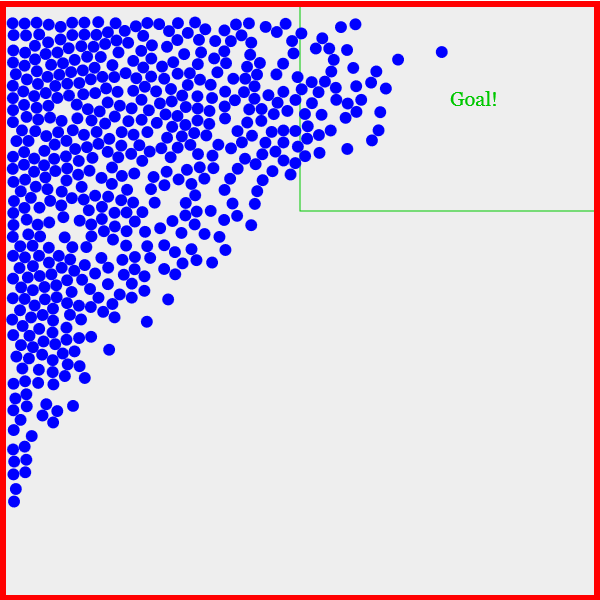
\includegraphics[width=4cm]{fig/500RobotBrown3}
\caption{Screen Shot of a run of 500 Robots with brownian noise.}
\end{center}
\end{figure}
\begin{figure}[h]
\begin{center}
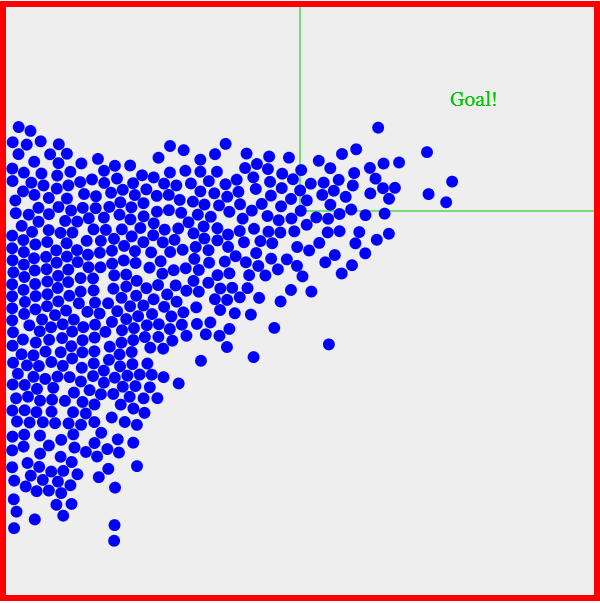
\includegraphics[width=4cm]{fig/500RobotBrown2}
\caption{Screen Shot of a run of 500 Robots with brownian noise after colliding the lower wall.}
\end{center}
\end{figure}
As we expected, we can see the Gaussian distribution when colliding the wall in \emph{y} axis.

\subsection{\emph{Mean Controllability Proof}}
\begin{itemize}
\item The plot of showing controllability:

\end{itemize}
\begin{figure}[h]
\begin{center}
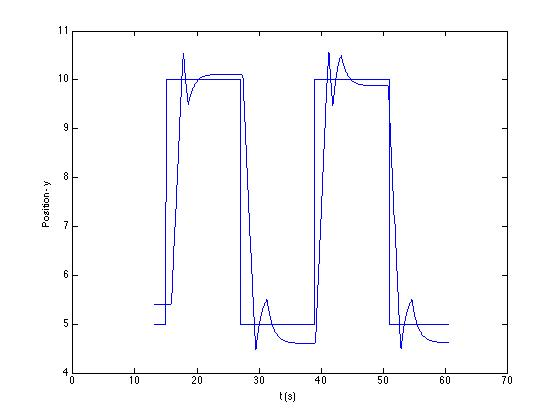
\includegraphics[width=10cm]{fig/PlotPosition}
\caption{During the time, we reach our goal approximately}
\end{center}
\end{figure}



\end{document}
